\title{Comparison of Sequential and Parallel Fast Fourier Transform}
\author{
	Rami Jurdi \\
	Zachary Noble \\
	Gregory Freitas \\
	Jayden Bendezu
}
\date{\today}

\documentclass[journal]{IEEEtran}
\usepackage[utf8]{inputenc}
\usepackage{amsmath}
\usepackage{graphicx}
\graphicspath{ {./images/} }

\begin{document}
\maketitle

\begin{abstract}
This research is in the Digital Signal Processing field 
where our aims are to improve the performance of real-time signal 
processing using parallel processing techniques coupled with 1 
dimensional Fast Fourier Transforms. 
It has been done before by other researchers implementing 
multi-dimensional Fast Fourier Transforms in a multi-threaded context. 
The purpose of our research is to gain a better understanding of 
parallel processing techniques and digital signal processing. 
Thus the main goal is to observe the outcome of implementing a 
multi-threaded Fast Fourier transform algorithm and learn from the 
state-of-the-art research.
\end{abstract}

\section{Introduction}
	\par {The Fast Fourier transform (FFT) is an algorithm that uses Discrete Fourier transforms
	 (DFT) on a time sequence to convert a signal, usually based on time, to a signal based in the
	 frequency domain. This allows us to analyze a sequence of time-values by decomposing it into 
	 bins of different frequencies. The Fast Fourier transform is used in many applications ranging 
	 from digital signal processing, sampling, pitch correction software, and wave analysis.}

	\par {The direct computation of the DFT results in $n^2$ multiplications and $n(n-1)$ additions, 
	making the computation greatly expensive for sufficiently large $n$.  Over the course of many years
	of research done by researchers in the field, more efficient algorithms were developed for computing DFTs,
	such as the Cooley-Tukey FFT algorithm. This algorithm reduces the time complexity of the computation of
	Fourier transforms from $O(n^2)$ to $O(nlogn)$~\cite{Xiang}}.

	\par {In this paper, we present our process of implementing the parallel FFT algorithm, specifically
	a variant of the Cooley-Tukey algorithm, and conduct performance comparisons between the sequential and 
	parallel versions of the algorithm in C++.}

\section{Target Problem}
	\par {The main problem at hand is to create an application that is able to process signals 
	provided to the program as audio files such as .WAV, .MP3, and .MP4. Then displaying the audio 
	files as a spectrograph of its signals, which is calculated using the Fast Fourier Transform
	algorithm. This problem can be broken into several steps of 
	what we need to achieve.}

\begin{itemize}
	\item A GUI to interact with.
	\item Accepting audio files via local upload.
	\item Decoding the raw audio file data.
	\item Computing the parallelized Fast Fourier Transform on the audio signal.
	\item Displaying the detected frequencies in a Frequency vs. Amplitude chart.
\end{itemize}

\subsection{Approach}\label{Approach}
	\par {Tackling some of the above sub-problems. In order to create a GUI to interact with, 
	we will write the program using the QT C++ GUI framework to simplify taking audio files 
	from disk and decoding the raw data. Through the use of provided libraries of QT the 
	basic functionality of loading files and playing/decoding audio is handled and we use 
	them on a higher level. This will allow us to focus more on the problem of processing 
	signals for the audio files. Then by handling extracting raw data from the audio files 
	using the QAudioDecoder class provided by QT, we intend to use one-dimensional Fast 
	Fourier Transforms to process the signals. (How do we plan to parallelize the FFT is 
	what would be discussed here briefly since will be explained thoroughly within 
	the algorithms subsection).}
\subsubsection{Project Architecture}


\subsection{Plan Outline}

\par{
	An outline of how our project development was structured is detailed below:
}
\begin{enumerate}
	\item Setup programming environment using Qt C++.
	\item Add support using Qt multimedia APIs to load and decode audio files from disk.
	\item Stream the audio data to an output device such as speakers or headphones.
	\item Display a waveform of the audio.
	\item Implement single-threaded Fast Fourier Transforms.
	\item Implement multi-threaded Fast Fourier Transforms.
	\item Display the frequency vs. amplitude data calculated from the Fast Fourier Transform, in order to validate correctness.
	\item Conduct experimental tests comparing multi-threaded implementation vs sequential implementation. 
Observe any performance boosts if any.
\end{enumerate}

\subsection{Algorithm}
	 
\subsubsection{Discrete Fourier Transform}
% can go into just what the discrete fourier transform is and its runtime and space complexity.
	\par{
		The Discrete Fourier Transform (DFT) can be calculated as 
		a summation of the product of the sample value and a complex
		exponential term, shown in equation (\ref{DFT1}).
	}
		\begin{equation}\label{DFT1}
			\displaystyle X_k = 
			\sum_{n=0}^{N-1}x_ne^{\displaystyle\frac{-j2 \pi kn}{N}}
		\end{equation}
	\par{
		Where $x_n$ denotes the sample value at index $n$, $j$ the imaginary
		number, $k$ the desired frequency, and $N$ the total number of samples.
		The output of the DFT $X_k$ is the Fourier Transform coefficient for
		frequency $k$, which in our program is the magnitude of the real 
		and imaginary output of the DFT, normalized between 0 and 1 with 1
		indicating a large response from the DFT for that frequency $k$.
	}
	\par{
		An equivalent summation can be derived in terms of the trigonemetric
		functions cosine and sine using Euler's Identity $e^{ix}=cosx + isinx$,
		as shown in equation (\ref{DFT2}).
	}
		\begin{equation}\label{DFT2}
			\displaystyle X_k = \sum_{n=0}^{N-1}x_n[cos(\frac{2\pi}{N}kn) 
			- jsin(\frac{2\pi}{N}kn)]
		\end{equation}

	\par{
		This version of the DFT makes it easier to compute the real and
		imaginary components of the equation in code through the use of 
		the std::complex class in the C++ STL.
	}

	\par{
		As mentioned in the introduction, the runtime complexity for direct
		computation of the DFT is $O(n^2)$ which makes it unusable in real-time
		applications for significantly large sample sizes; however, the main
		idea behind the DFT computation is used in the FFT algorithm, but the 
		computation is repeatedly sub-divided instead, 
		achieving better overall performance.
	}

	%\par While we established that we will be using the Fourier Transforms. As the base implementation of fourier transforms resolves to a $O(n^2)$ runtime according to~\cite{Xie}.
\subsubsection{Fast Fourier Transform}
% can go into just what the fast fourier transform is and its runtime and space complexity.
	\par {
		It is essential that we use an implementation that yields a 
		better runtime as in the case of our program, operating on 
		larger audio files will begin to take much longer and become more 
		inefficient. Thus we will be working with the 
		Fast Fourier transform algorithm to reduce our upper 
		asymptotic bound. The specific FFT algorithm we used is the Cooley-Tukey 
		radix-2 Decimation in Time (DIT) algorithm, which repeatedly divides a 
		DFT of size $N$ into two interleaved DFTs of size $N / 2$.
	}
	\par{
		The interleaving of DFTs is achieved by splitting the even-indexed samples
		and odd-indexed samples of the original $N$ sized DFT, computing them using
		the DFT formula, and combining the results to produce the DFT of the 
		original signal. This assumes that the original DFT size $N$ is a 
		power of 2, which can be ensured by using zero-padding in applications 
		where the original audio file might not be a power of 2.
		A visualization of how the input signal is divided in the Cooley-Tukey
		radix-2 DIT algorithm is shown in Figure \ref{fig:dft-decomp}.
	}
	\begin{figure}[h]
		\centering
		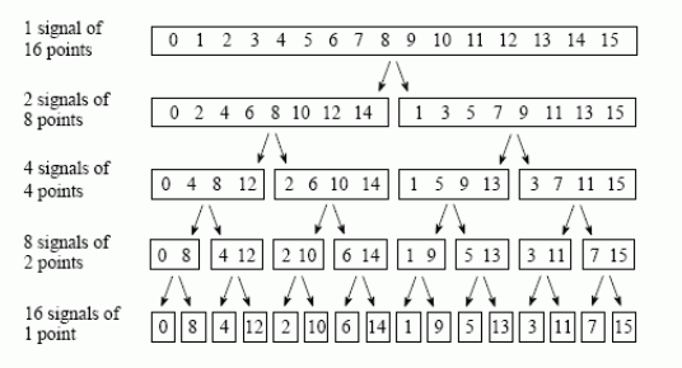
\includegraphics[width=0.5\textwidth]{dft-decomp}
		\caption{Example of interleaved decomposition of a 16 point input signal
		\cite{DspGuide}.}
		\label{fig:dft-decomp}
	\end{figure}

	\par{
		The first level of splitting of the DFT
		can be written as two summations, one
		operating on even-indices and one on 
		odd indices, as show in equation (\ref{FFT}).

		\begin{equation}\label{FFT}
			\displaystyle X_k = \sum_{n=0}^{\frac{N}{2} - 1}x_{2n}e^{\displaystyle\frac{-j2\pi k(2n)}{N}}
			+ \sum_{n=0}^{\frac{N}{2} - 1}x_{2n + 1}e^{\displaystyle\frac{-j2\pi k(2n + 1)}{N}}
		\end{equation}
	}

	\par{
		This equation is simplified in terms of cosine and sine for code
		simplicity in the implementation, similar to equation (\ref{DFT2}).
		The algorithm for the Cooley-Tukey radix-2 DIT algorithm also makes
		use of bit-reversal permutation addressing, which swaps the
		real/imaginary signal input elements based on the bit reversal of their
		respective index in the signal. This is needed because the splitting
		of even/odd index elements in the calculation of the FFT leads to 
		unordered output, which this permutation can prevent by pre-processing
		the bit-reversals in $O(n)$ runtime. Overall, the runtime for the
		FFT is $O(nlogn)$, which is a significant improvement from the $O(n^2)$
		runtime from the direct computation of the DFT.

		The sequential implementation in C++ of the Cooley-Tukey radix-2 DIT
		algorithm that we used in our application came from Project Nayuki 
		\cite{Nayuki} and was modified for our use-case.
	}
\subsection{Parallelized Fast Fourier Transform}
% Can specify more on how the threads will interact with the fourier transform, 
% why the number of threads we chose and such.
		\par{
			As explained in section \ref{Approach}, our application implements
			a DistributedFFTWorkerThread class which computes the FFT on a
			slice of the original input of size $N$. This implementation makes use
			of the QThread API from the Qt 5 C++ core library. We decided to use 8
			total FFT worker threads with each thread operating on an evenly-split
			amount of samples, padded to the next power of 2 if needed, using
			bit-shifting to find the size and resizing the std::vector, padded with
			0s.

			Each thread is spawned in the FTController class which assigns each thread
			a unique ID from 0-7, which is used in the range calculation
			(\ref{RangeEq}) of the indices to calculate the FFT on. 
			
			\begin{equation}\label{RangeEq}
				data_i = signal[i*N/p, (i+1)*N/p - 1] (i = 0, ..., p-1)
			\end{equation}

			Where $N$ is the total size of the $signal$ input array,
			$i$ is the unique worker ID, and $p$ is the total amount of worker
			threads.

			This range calculation (\ref{RangeEq}) is a relatively common
			approach to distributing work between multiple threads, allowing for
			concurrent work to be done, and was used in the research paper by 
			Zhong Cui-xiang et al. \cite{Xiang}, in which they utilize a 
			multiprocessor system to speed up the computation of the 1-D
			FFT radix-2 DIT algorithm.

			For our approach we only utilize threads which operate on separate
			sections of the signal input, ensuring thread-safe computation
			without the use of any mutual-exclusion locks. Each thread, however,
			needs to relay the computed output back to the FTController through
			the use of thread-safe signals available in the Qt Core library, 
			which could lead to a potential bottleneck for a greater amount of
			threads. Finally, the FTController combines the split output of the worker
			threads into a local vector of (frequency, magnitude) points, which
			is used to plot the Frequency vs. Amplitude graph in our application.
		}

\subsection{Experimental Results}
	\par{
		Below is our performance results of the sequential and parallel
		implementations of the Fast Fourier Transform
		tested on three different WAV audio files. The computation
		time may vary among different systems due to hardware capabilities.
	}

\vspace{1em}
\hspace{-1em}
\begin{tabular} { |c|c|c|c| }
	\hline
	\multicolumn{4} {|c|} {Data Set 1} \\
	\hline
	Algorithm & File & File Size & Comp. Time \\
	\hline
	Sequential FFT & 440Hz-1s.wav & 88 KB & 0.0051s \\
	Parallel FFT & 440Hz-1s.wav & 88 KB & 0.0014s \\
	\hline
\end{tabular}

\vspace{1em}
\hspace{-1em}
\begin{tabular} { |c|c|c|c| }
	\hline
	\multicolumn{4} {|c|} {Data Set 2} \\
	\hline
	Algorithm & File & File Size & Comp. Time \\
	\hline
	Sequential FFT & 440Hz-3s.wav & 260 KB & 0.023s \\
	Parallel FFT & 440hz-3s.wav & 260 KB & 0.0047s \\
	\hline
\end{tabular}

\vspace{1em}
\hspace{-1em}
\begin{tabular} { |c|c|c|c| }
	\hline
	\multicolumn{4} {|c|} {Data Set 3} \\
	\hline
	Algorithm & File & File Size & Comp. Time \\
	\hline
	Sequential FFT & 440Hz-30s.wav & 2.5 MB & 0.34s \\
	Parallel FFT & 440Hz-30s.wav & 2.5 MB & 0.058s \\
	\hline
\end{tabular}

	\vspace{1em}
	\par{
		The last data set, which contains the 440Hz-30s.wav file, has over
		1.3 million total samples in the signal, which is sufficient enough
		to compare runtimes of the sequential/parallel FFT algorithms. Each
		audio file was sampled at 44100 Hz, with a 16 bit sample size. So, a 30
		second audio file sampled at 44100 Hz contains $30 * 44100 = 1323000$
		total samples, which is used as input for the parallel/sequential FFT.
	}
	\par{
		Additionally, each audio file had its FFT computed for 50 trials each, 
		for both the sequential and parallel FFT algorithms, and the 
		average runtimes were calculated and are displayed in the Comp. Time 
		column in the table above. We observed a speedup factor of 
		around 6x on the 30s audio file, utilizing 8 worker threads with our 
		parallel FFT algorithm. As the number of samples increase, 
		there is a greater performance increase between the sequential and 
		parallel FFT implementations, as can be observed in the table.
	}

\section{State-of-the-Art Research}

	\par {
		The discrete fourier transforms have a variety of applications for the 
		science and engineering fields \cite{Xiang}.Though due to how inefficient 
		the base form of fourier transforms are, the cooley tukey fast fourier transform 
		was developed in 1965 that was later expanded on \cite{CTA}. These modified implementations 
		make up the state of the art research in digtial signal processing using fourier transforms. 
		Although there are several implemenations, they are typically those that improve on the constant 
		factors, none of which that obtain a better upper asymptotic bound of ${O(N Log(N))}$. The different 
		algorithms are explained in more detail in the following sub sections.
	}
	% Within each after describing the algorithms key difference I will elaborate on oppurtunities to parallelize,
	% and reference papers that do parallelize the algorithm.
	% Should state of the art talk about the different overall approaches to parallelizing these algorithms, such as
	% communications between threads, or indpendantly computing calculations.

	\subsection{Radix 2 Decimation in Time}
		% Is it acceptable to use abbreviations?
		\par{
			This RAD 2 DIT algorithm makes use of the divide and conquer methodology. Through exploiting 
			the symmetrical properties of the DFT the summation can be broken up into computations of even 
			and odd sample points \cite{Soni}. The sub trees of even and odd points are then continuously 
			broken up into smaller transforms. Due to the computations calculate not being in a natural ordering 
			it is necessary to use bit reversal to obtain the natural ordering of the results.
		}
		\par{
			There is a parallel implementation of the RAD2 DIT algorithm utilized 
		}
	\subsection{Split Radix FFT}
		\par{

		}
	\subsection{Bluestein's Algorithm}
		\par{

		}

\subsection{Related Work}
\par{
	Will talk about how our implementation comapares
}

\section{Our Contributions}

\medskip
\bibliographystyle{ieeetr}
\bibliography{report.bib}

\end{document}



